\documentclass[12pt,a4paper]{report}
\usepackage[utf8]{vietnam}
\usepackage[utf8]{inputenc}
\usepackage{tabto}
\usepackage{amsmath}
\usepackage{amsfonts}
\usepackage{multicol}
\usepackage{tikz}
\usepackage{amssymb}
\usepackage{listings}
\usepackage[left=2cm,right=2cm,top=2cm,bottom=2cm]{geometry}
\usepackage{graphicx}
\graphicspath{ {./images/} }
\author{Trần Đức Mạnh}
\title{Sequence Models}

\begin{document}
\maketitle
\tableofcontents

\chapter{Recurrent Neural Networks}
	\section{Recurrent Neural Networks}
		\subsection{Notation}
			\begin{itemize}
				\item $x$: chuỗi input
				\item $y$: chuỗi output
				\item $x^{(i)<t>}, y^{(i)<t>}$: từ thứ $t$ của chuỗi input/output trong example thứ $i$. Là một \textbf{one-hot vector} (Tức là vector mà chỉ có 1 phần tử nào đó bằng 1, còn lại bằng 0)
					\begin{equation}
						x^{<t>} = 
						\begin{bmatrix}
							0\\
							0\\
							\vdots\\
							0\\
							1\\
							0\\
							\vdots\\
							0						
						\end{bmatrix}
					\end{equation}
				\item $T_{x}^{(i)}, T_{y}^{(i)}$: độ dài của chuỗi input/output trong example thứ $i$
				\item Vocabulary: từ điển từ, một String Array
					\begin{equation}
						\text{vocabulary} = 
						\begin{bmatrix}
							\text{a}\\
							\text{aaron}\\
							\vdots\\
							\text{zulu}						
						\end{bmatrix}
					\end{equation}
				\begin{itemize}
					\item \textbf{Lưu ý}: $x^{<t>}$ có chiều bằng vocabulary, và có phần tử tại vị trí tương ứng với vocabulary bằng 1
					\item Ví du: Trong Vocabulary, từ "and" ở vị trí 367, thì $x^{<t>}$ tương ứng với "and" sẽ là một one-hot vector, với phần tử thứ 367 bằng 1	
				\end{itemize}
			\end{itemize}
		\subsection{Recurrent Neural Network Model}
			\begin{itemize}
				\item Tại sao không sử dụng Standard network?
					\begin{itemize}
						\item Vì độ dài chuỗi input và chuỗi output có thể khác nhác nhau với mỗi examples.
						\item Vì chúng ta có quan tâm tới thứ tự của từ trong chuỗi, và Standard network không xử lý được thông tin ý
					\end{itemize}					 
				\item Recurrent Neural Network
					\begin{figure}[h]
						\caption{RNN Model}
						\centering
					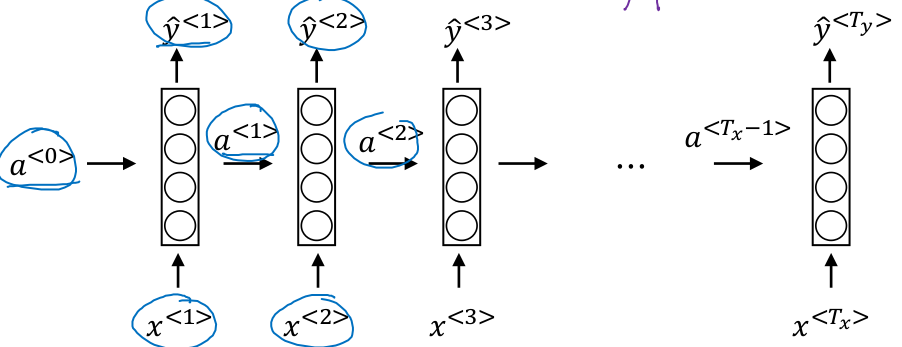
\includegraphics[width=0.5\textwidth]{1}
					\end{figure}
					\begin{itemize}
						\item Forward:
							\begin{itemize}
								\item $a^{<t>} = g(\omega_{aa} a^{<t-1>} + \omega_{ax} x^{<t>} + b_a) = g(\omega_a[a^{<t-1>}, x^{<t>}] + b_a)$
								\item $\hat{y}^{<t>} = g(\omega_{ya} a^{<t>} + b_y) = g(\omega_{y} a^{<t>} + b_y)$
									\begin{itemize}
										\item $\omega_{ax}$: weight tính cho $a$ và nhân với $x$ (tương tự: $\omega_{ya}$ là weight tính cho $y$ và nhân với $a$)
										\item $b_a$: bias tính cho $a$ (tương tự: $b_y$: bias tính cho $y$)
										\item $\omega_{aa} a^{<t-1>} + \omega_{ax} x^{<t>} = \omega_a[a^{<t-1>}, x^{<t>}]$
										\item $\omega_a = [\omega_{aa} \vdots \omega_{ax}]$ (tức là ghép $\omega_{aa} (a, b)$ với $\omega_{ax} (a, c)$ thành $\omega_a (a, b + c)$)
										\item $[a^{<t-1>}, x^{<t>}] = \begin{bmatrix}
										a^{<t-1>}\\
										x^{<t>}
										\end{bmatrix}$\\ (tức là ghép $a^{<t-1>} (n, 1)$ với $x^{<t>} (m, 1)$ thành $\begin{bmatrix}
										a^{<t-1>}\\
										x^{<t>}
										\end{bmatrix} (n + m, 1)$)
									\end{itemize}
							\end{itemize}
					\end{itemize}
			\end{itemize}
		\subsection{Different types of RNNs}
			\begin{itemize}
				\item One to one:\\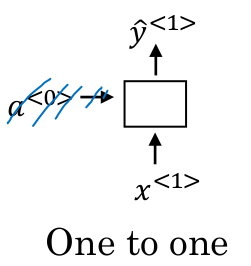
\includegraphics[width=0.2\textwidth]{1to1}
				\item One to many:\\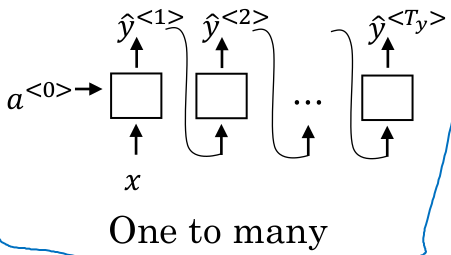
\includegraphics[width=0.5\textwidth]{1toMany}
				\item Many to one:\\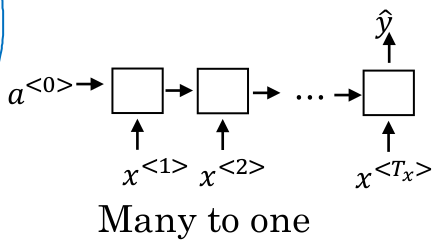
\includegraphics[width=0.5\textwidth]{ManyTo1}
				\item Many to many ($T_x=T_y$):\\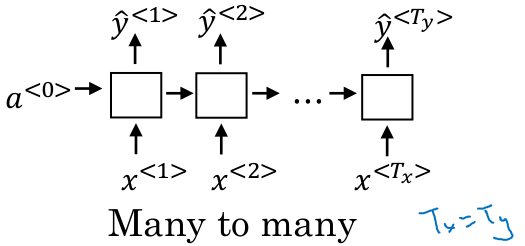
\includegraphics[width=0.5\textwidth]{ManyToMany1}
				\item Many to many (Sequence to Sequence):\\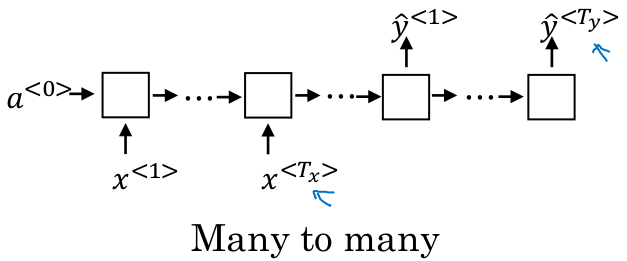
\includegraphics[width=0.5\textwidth]{ManyToMany2}
			\end{itemize}
		\subsection{Language model and sequence generation}
		\subsection{Vanishing gradients with RNNs}
		\subsection{GRU}
			\begin{itemize}
				\item Hình ảnh minh họa:\\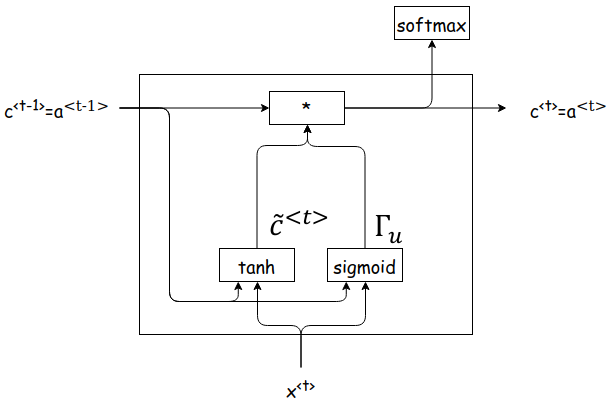
\includegraphics[width=0.5\textwidth]{GRU}
				\item Chi tiết:
					\begin{itemize}
						\item $\tilde{c}^{<t>}=tanh(\omega_c[\Gamma_r*c^{<t-1>},x^{<t>}]+b_c)$
						\begin{itemize}
												\item $\Gamma_r = \sigma(\omega_r[c^{<t-1>},x^{<t>}]+b_r)$
						\end{itemize}
						\item $\Gamma_u = \sigma(\omega_u[c^{<t-1>},x^{<t>}]+b_u)$
						\item $c^{<t>}=\Gamma_u*\tilde{c}^{<t>} + (1 - \Gamma_u) * c^{<t-1>}$ (tính toán ở hộp *)
					\end{itemize}
			\end{itemize}
		\subsection{LSTM}
			\begin{itemize}
				\item Hình ảnh minh họa:\\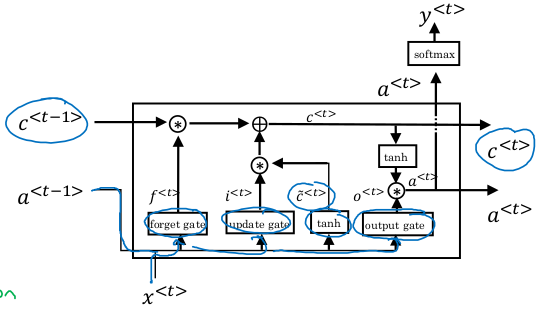
\includegraphics[width=0.5\textwidth]{LSTM}
				\item Chi tiết:
					\begin{itemize}
						\item $\tilde{c}^{<t>}=tanh(\omega_c[a^{<t-1>},x^{<t>}]+b_c)$
						\item $\Gamma_u = \sigma(\omega_u[a^{<t-1>},x^{<t>}]+b_u)$
						\item $\Gamma_f = \sigma(\omega_f[a^{<t-1>},x^{<t>}]+b_f)$
						\item $\Gamma_o = \sigma(\omega_o[a^{<t-1>},x^{<t>}]+b_o)$
						\item $c^{<t>}=\Gamma_u*\tilde{c}^{<t>} + \Gamma_f * c^{<t-1>}$
						\item $a^{<t>} = \Gamma_o * tanh(c^{<t>})$
					\end{itemize}
			\end{itemize}
		\subsection{Bidiractional RNN}
			\begin{itemize}
				\item RNN 2 chiều đưa ra để giải quyết hạn chế của RNN 1 chiều trong việc lấy thông tin của chuỗi. RNN 1 chiều chỉ có thể trích thông tin từ "quá khứ", trong khi thông tin từ "tương lai" cũng quan trọng không kém.
				\item Hình ảnh mình họa:\\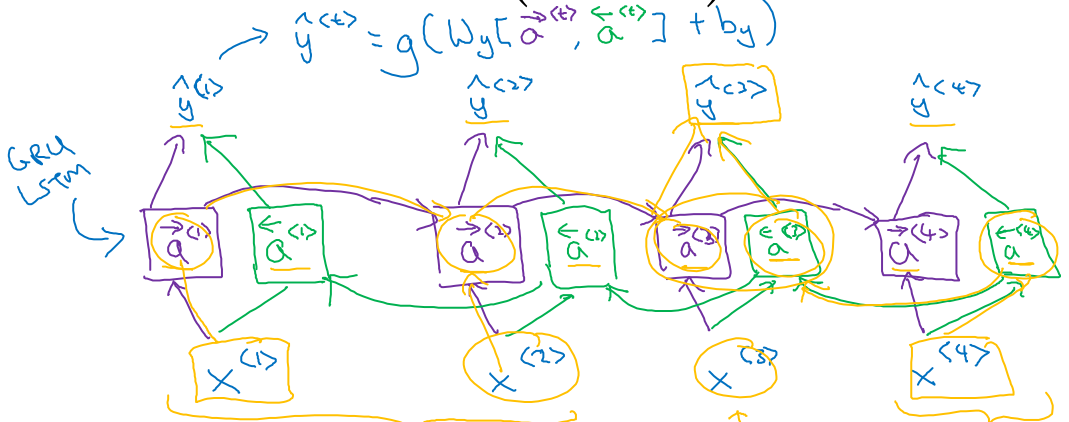
\includegraphics[width=0.7\textwidth]{BiRNN}
			\end{itemize}
		\subsection{Deep RNNs}
\chapter{Natural Language Processing \& Word Embeddings}
	\section{Introduction to Word Embeddings}
		\subsection{Word Representation}
			\begin{itemize}
			\item Tại sao one-hot vector chưa đủ tốt?
				\begin{itemize}
				\item Đặt vấn đề: Bạn có 1 chuỗi "I want orange \dots", và Model của bạn học được rằng "juice" là từ thích hợp để điền vào \dots, tuy nhiên điều đó không có nghĩa rằng Model của bạn cũng biết điền "juice" vào nếu chuỗi là "I want apple \dots". Điều này xảy ra vì one-hot vector không thể hiện sự tương đồng giữa "orange" và "juice".
				\item Đề khắc phục điều đó, chúng ta sử dụng \textbf{Featurized Representation} thay cho One-Hot.
				\end{itemize}
			\item Featurized Representation: Word embedding
				\begin{figure}[h]
					\caption{Ví dụ:}
					\centering
					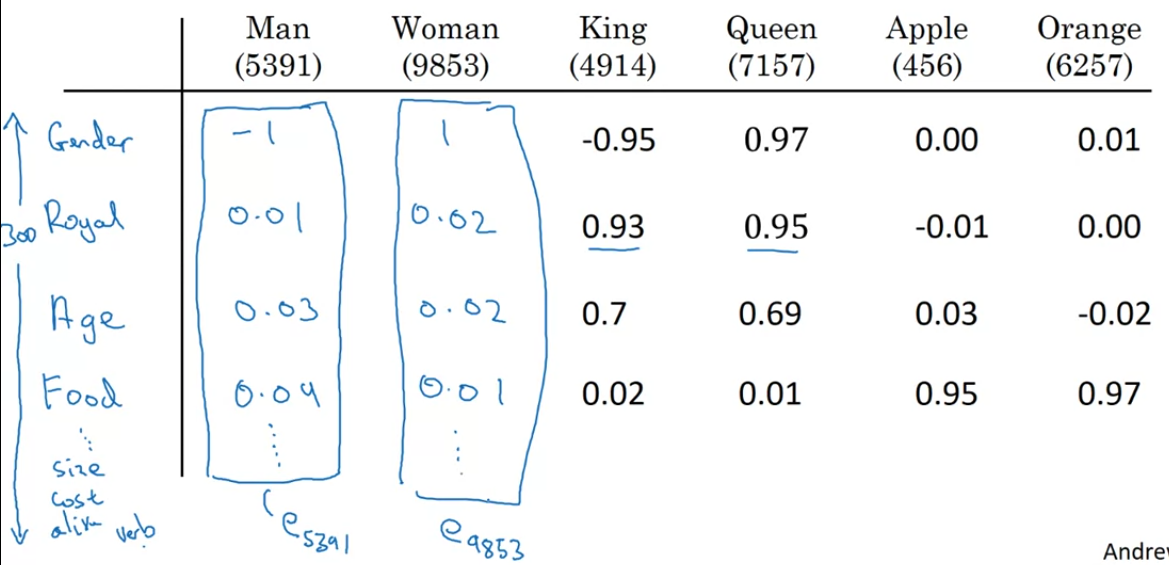
\includegraphics[width=0.7\textwidth]{2}
				\end{figure}
				\begin{itemize}
				\item Nhận xét ví dụ:
					\begin{itemize}
					\item Vì one-hot vector chỉ có thể chỉ vị trí của từ trong Vocabulary \textit{(như Man(5391) là để chỉ từ "Man" nằm ở vị trí 5391 trong Vocabulary)}, nên ta sử dụng Featurized Representation để có thể thể hiện cả những tính chất của từ.
					\item Bằng cách này, ta thấy rõ Man và Woman khá tương đồng nhưng chỉ khác nhau rõ rệt về Gender, còn Apple và Orange lúc này có các chỉ số gần như giống nhau, hay nói cách khác là lúc này ta đã biểu diễn được 2 từ này một cách tương đồng nhau hơn
					\item $e_{5391}$ là để chỉ vector tương ứng với từ 5391 trong Vocabulary \textit{(trường hợp này là "Man")}, còn $O_{5391}$ là để chỉ one-hot vector của từ đó
					\end{itemize}
				\end{itemize}
			\item Visualizing Word Embeddings
			\end{itemize}
		\subsection{Using Word Embeddings}
		\subsection{Properties of Word Embeddings}
		\subsection{Embedding Matrix}
			\begin{itemize}
			\item Gọi $E$ là Embedding Matrix, ta có: $E \times O_t = e_t$ ($(m, n) \times (n, 1) = (m, 1)$)
				\begin{itemize}
				\item $m$: số lượng features
				\item $n$: số lượng từ trong Vocabulary
				\item $t$: Vị trí của từ trong Vocabulary
				\end{itemize}
			\end{itemize}
			\begin{figure}[h]
					\caption{Hình ảnh minh họa:}
					\centering
					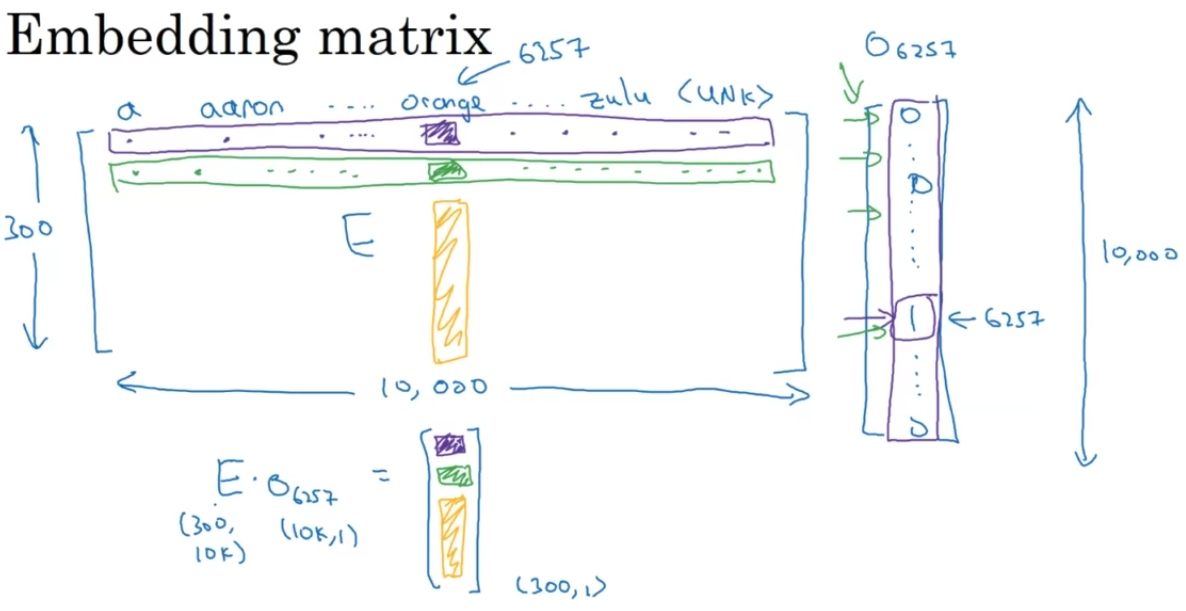
\includegraphics[width=0.8\textwidth]{3}
				\end{figure}
	\section{Learning Word Embeddings: Word2Vec \& Glove}
		\subsection{Learning Word Embeddings}
			\begin{itemize}
			\item Neural Language Model
				\begin{figure}
					\caption{Neural Language Model}
					\centering
					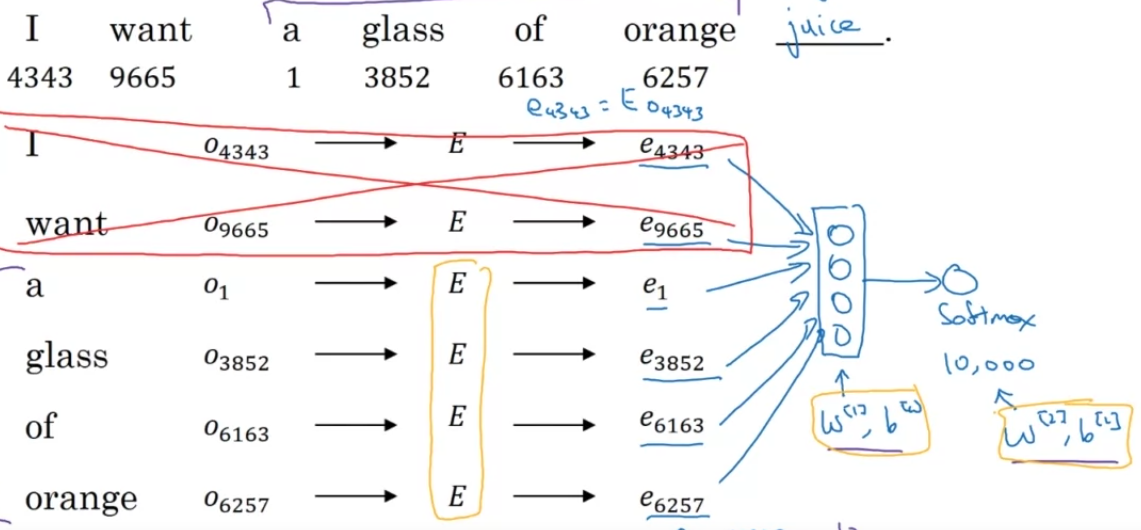
\includegraphics[width=0.7\textwidth]{4}
				\end{figure}
				\begin{itemize}
				\item Ở hình 2.3, với context "I want a glass of orange \dots" và ta muốn Model này điền "juice" vào chỗ \dots
				\item Để làm được điều đó, xây dựng Model theo hình 2.3 và cho nó học 5 parameters sau: $E, \omega^{[1]}, b^{[1]}, \omega^{[2]}, b^{[2]}$
				\item Thay vì sử dụng tất 7 kí tự của chuỗi được cho, ta có thể chỉ sử dụng 5 kí tự gần \dots để làm context
				\end{itemize}
			\item Other context/target pair
				\begin{itemize}
				\item Cho ví dụ: I want a glass of orange  \underline{juice} to go along with my cereal.
				\item Context/target pair:
					\begin{itemize}
					\item Last 4 words: "a glass of orange \underline{   ?   }"
					\item 4 words on left \& right: "a glass of orange \underline{   ?   } to go along with"
					\item Last 1 word: "orange \underline{   ?   }"
					\item Nearby 1 word \textbf{(skip gram)}: "glass \dots \underline{   ?   }"	
					\end{itemize}
				\end{itemize}
			\end{itemize}
		\subsection{Word2Vec}
			\begin{itemize}
			\item Skip-grams model
				\begin{itemize}
				\item Ý tưởng: Model này chọn 1 từ làm Context, rồi chọn 1 từ làm Target \textit{(có nhiều cách chọn, nhưng ngày gần, cách 1 từ, cách 10 từ, \dots)}, rồi cho Model này học cách dự đoán Target từ Context. Nhưng mục đích của Model này không phải là để dự đoán chính xác Target mà là để \textbf{học Embedding Matrix $E$}.
				\item Model: 
					\begin{itemize}
					\item Với Vocab Size = 10000, Context c và Target c, ta có:
					\item $O_c \rightarrow E \rightarrow e_c \rightarrow \text{(Softmax)} \rightarrow \hat{y}$
					\item Softmax: $P(t|c)=\frac{e^{\theta^T_t e_c}}{\sum^{10000}_{j=1}e^{\theta^T_j e_c}}$ với $\theta_t = $ parameter của output $t$
					\item Cost: $L(\hat{y},y)=-\sum_{i=1}^{10000}y_ilog(\hat{y}_i)$
					\end{itemize}
				\end{itemize}
			\item Problem with softmax classification
				\begin{itemize}
				\item $P(t|c)=\frac{e^{\theta^T_t e_c}}{\sum^{10000}_{j=1}e^{\theta^T_j e_c}}$ có Computation Cost cao vì tổng của 10000 khá lớn, và sẽ càng tốn nếu vocab size của bạn càng lớn.
				\item Cách giải quyết:
					\begin{itemize}
					\item Hierarchy Softmax
					\end{itemize}
				\end{itemize}
			\end{itemize}
		\subsection{Negative Sampling}
			\begin{itemize}
			\item Ý tưởng: là 1 Model khác được đưa ra nhằm giải quyết vấn đề computation cost của Skip-grams.\\ Model này học cách nhận 1 cặp từ và đoán xem nó có đúng là 1 cặp context/target hay không.
			\item Dataset:
				\begin{itemize}
				\item Dataset này được tạo ra bằng cách chọn 1 từ làm Context, rồi chọn 1 từ làm Target, label cặp từ này là 1. Rồi chọn $K$ từ khác từ Vocabulary để làm Target rồi label K cặp này là 0.
				\item Ví dụ: (word ở đây là Target, còn target? là label)\\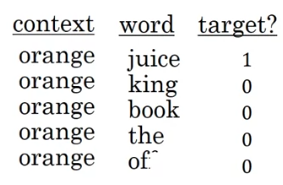
\includegraphics[width=0.5\textwidth]{5}
					\begin{itemize}
					\item Small Dataset: $K = [5;20]$
					\item Large Dataset: $K = [5;20]$
					\end{itemize}
				\item Cách chọn $K$ từ để label 0 (Negative Sample): \textbf{(Chưa hiểu lắm)}
				\end{itemize}
			\item Model:
				\begin{itemize}
				\item $O_c \rightarrow E \rightarrow e_c \rightarrow \begin{matrix}
				O\\
				O\\
				\vdots\\
				O
				\end{matrix}$
				\item Layer cuối của model là 10000 binary classification, mỗi node trả lời câu hỏi tương ứng (juice? king? \dots)
				\item Mỗi node lúc này tính toán: $P(y=1|c, t)=\sigma(\theta^T_te_c)$ với với $\theta_t = $ parameter của output $t$
				\item Với mỗi iteration: 
					\begin{itemize}
					\item Ta train $K+1$ node (kèm với $E$)
					\item Chọn $K$ negative sample khác rồi train model
					\end{itemize}
				\item Vì thay vì train 10000 node, giờ ta chỉ train $K+1$ nên computation cost rẻ hơn rất nhiều
				\end{itemize}
			\end{itemize}
		\subsection{GloVe Word Vectors}
			\begin{itemize}
			\item \textbf{I don't thing this is important to fully understand}
			\end{itemize}
	\section{Applications Using Word Embeddings}
		\subsection{Sentiment Classification}
		\subsection{Debiasing Word Embeddings}
\chapter{Seuqence Models \& Attention Mechanism}
	\subsection{Basic Model}
	\subsection{Picking the Most Likely Sentence}
		\begin{itemize}
		\item Trong Machine Translation \textit{(hay những bài toán tương tự)}, chúng ta có thể có được nhiều hơn 1 chuỗi Output từ 1 chuỗi input, thì vấn đề ở đây là chúng ta không thể chọn bừa 1 trong những chuỗi Output đó \textit{(vì trong số đó chắc chắn có chuỗi Output phù hợp hơn các chuỗi còn lại, ví dụ có nhiều cách dịch từ ngôn ngữ đích sang ngôn ngữ nguồn, nhưng chắc chắn sẽ có cách dịch tốt hơn là chỉ dịch word-by-word)}. Chính vì thế mà ta phải tìm cách \textbf{"Picking the Most Likely Sentence"}.
		\item Bài toán được hiểu như sau: chọn output $y=y^{<1>},y^{<2>},\dots,y^{<T_y>}$ sao cho \break $P(y^{<1>},y^{<2>},\dots,y^{<T_y>}|x)$ là lớn nhất
			\[\text{arg} \max_{y^{<1>},\dots,y^{<T_y>}}P(y^{<1>},\dots,y^{<T_y>}|x)\]
		\item Một trong những cách không nên làm là \textbf{Greedy Search}:
			\begin{itemize}
			\item Thuật toán: chọn từng từ, sao cho nó là tốt nhất. Chọn $y^{<1>}$ sao cho nó là tốt nhất rồi chọn $y^{<2>}$ sao cho nó là tốt nhất rồi cứ thế đến $y^{<T_y>}$
			\item Lý do nó không tốt: 
				\begin{itemize}
				\item Cho 2 ví dụ sau:\\
				\tabto{0.5cm}Ví dụ 1: I am visiting Frence\\
				\tabto{0.5cm}Ví dụ 2: I am going to visiting Frence\\
				\tabto{0.5cm}Với $P(y|x)$ của ví dụ 1 tốt hơn
				\item Nhưng vì $P(\text{I am visiting}|x) < P(\text{I am going}|x)$ do "going" phổ biến hơn "visiting", nên Ví dụ 2 sẽ được chọn thay vì Ví dụ 1
				\end{itemize}
			\end{itemize}
		\end{itemize}
	\subsection{Beam Search}
		\begin{itemize}
		\item Thuật toán: Sau khi chạy Encoder, ở Decoder, sau khi tìm ra $\hat{y}^{<1>}$, tức tính được $P(\hat{y}^{<1>}|x)$ \textit{(là vector có chiều bằng Vocab Size, với mỗi phần tử là xác suất từ đó xuất hiện ở đầu câu)}. từ $P(\hat{y}^{<1>}|x)$ ta chọn ra $B$ \textbf{(Beam Width)} từ với xác suất cao nhất, lưu vào bộ nhớ.\\Rồi với mỗi từ được lưu trong bộ nhớ, ta tính $\hat{y}^{<2>}$ (ở đây tạo ra $B$ mạng để tính), ta được $P(\hat{y}^{<2>}|x,\hat{y}^{<1>})$, rồi ta tính $P(\hat{y}^{<1>},\hat{y}^{<2>}|x) = P(\hat{y}^{<1>}|x)P(\hat{y}^{<2>}|x,\hat{y}^{<1>})$ để từ đó chọn tiếp $B$ từ với xác suất $P(\hat{y}^{<1>},\hat{y}^{<2>}|x)$ cao nhất để tính $\hat{y}^{<3>}$
		\end{itemize}
	\subsection{Refinements to Beam Search}
		\begin{itemize}
		\item Ta có: \[\text{arg} \max_{y}P(y^{<1>},\dots,y^{<T_y>}|x) = \text{arg} \max_{y}\prod^{T_y}_{t=1}P(y^{<t>}|x,y^{<1>},\dots,y^{<t-1>})\]
		\item Ta có thể thấy tích $P(y^{<t>}|x,y^{<1>},\dots,y^{<t-1>})$ có thể trở nên rất nhỏ đến mức máy tính không thể lưu chính xác.\\Nên chúng ta tính toán bằng biểu thức tương tự sau:
		\[\text{arg} \max_{y}\sum^{T_y}_{t=1}logP(y^{<t>}|x,y^{<1>},\dots,y^{<t-1>})\]
		Bằng cách tính $log$ của xác suất, ta sẽ không phải lo về việc tràn số, đồng thời vẫn dữ nguyên được bản chất của phép toán.\\
		Tuy nhiên vẫn có thể xảy ra trường hợp tích xác suất quá nhỏ, dẫn đến giá trị $log$ bị âm rất lớn, dẫn đến tràn số, thì ta thêm $\frac{1}{T_y^{\alpha}}$ để ngăn điều đó.
		\[\frac{1}{T_y^{\alpha}}\sum^{T_y}_{t=1}logP(y^{<t>}|x,y^{<1>},\dots,y^{<t-1>})\]
		Trong đó $\alpha$ là hyperparameter, mục đích của $\alpha$ chỉ là để làm "mềm" phép tính (với $\alpha = 0.7$). Trong trường hợp $\alpha = 1$ là Length Normalize, còn $\alpha = 0$ là No Normalize.
		\end{itemize}
	\subsection{Error Analysis in Beam Search}
		\begin{itemize}
		\item
		\item
		\end{itemize}
	\subsection{Bleu Score}
	\subsection{Attention Model Intuition}
	\subsection{Attention Model}
\chapter{Transformer Network}

\end{document}
